\subsection{Pantalla de oficios salientes}
\subsubsection{Descripción}
%Descripción amplia de las funciones de la pantalla incluyendo la descripción de todos los botones y las validaciones con las que cuenta
	En esta pantalla se muestra el concentrado de todos los oficios salientes que se han registrado, mostrando su número de oficio, la dependencia que lo emitió, el asunto, la fecha de emisión y las acciones del oficio. La figura \ref{fig:OficiosSalientes} muestra el diseño de esta pantalla.			
		
	\begin{figure}[htbp!]
		\centering
			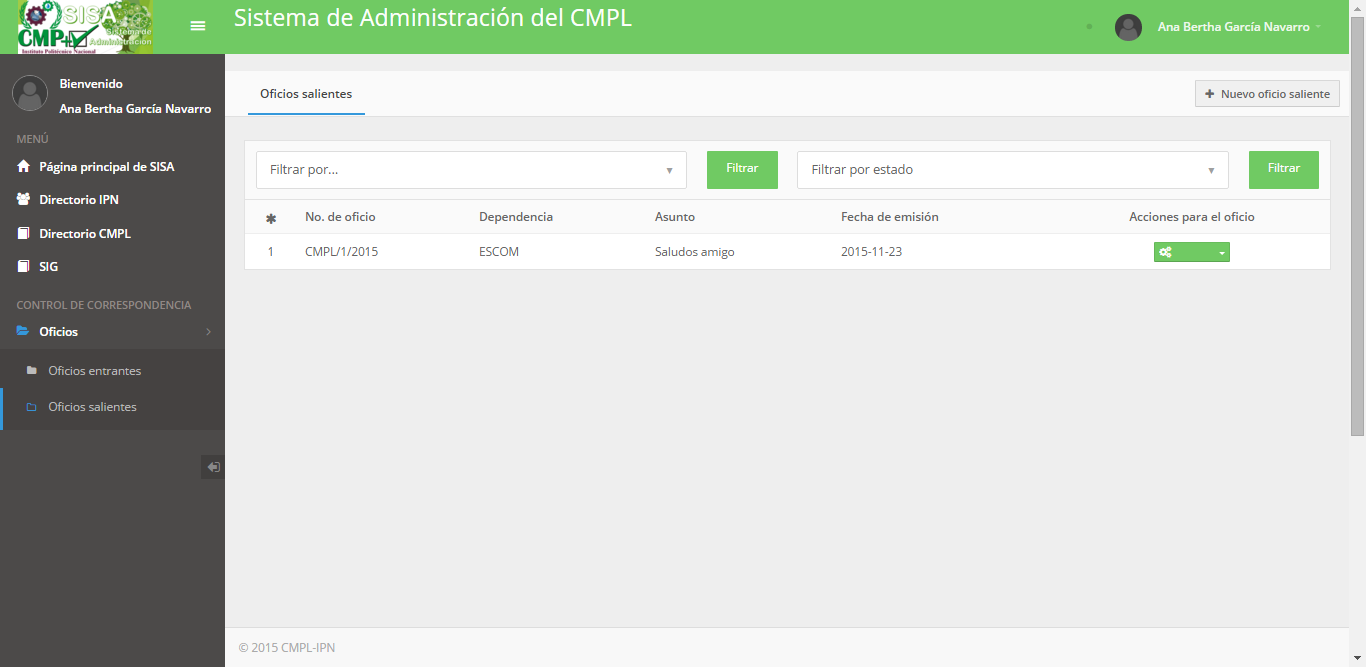
\includegraphics[width=1\textwidth]{Pantallas/OficiosSalientes.png}
		\caption{Pantalla de oficios salientes.}
		\label{fig:OficiosSalientes}
	\end{figure}

\subsubsection{Funcionamiento}
	Esta pantalla funciona de la siguiente manera:
	
	\begin{enumerate}
		\item El usuario puede seleccionar el tipo de filtro que mejor le convenga, y sea por consecutivo, por fecha de recepción, por dependencia o por estado.
		\item El usuario le da clic en ``Filtrar''.
		\item La aplicación aplica el filtro.
		\item La aplicación muestra los oficios salientes con el filtro correspondiente.
	\end{enumerate}

\subsubsection{Problemas que resuelve}
Esta pantalla ayuda a mitigar las causas que dan origen a los siguientes problemas:

	\begin{itemize}
		\item No se sabe cuál es el estatus de los oficios.
		\item El registro de los oficios no se lleva de forma correcta.
		\item Es complicado saber el orden de llegada de los oficios entrantes.
		\item No se sabe si ya se ha emitido una respuesta para el oficio.
		\item No se sabe quien fue el encargado de dar respuesta al oficio.
	\end{itemize}

\subsubsection{Pantallas relacionadas}
Está pantalla se relaciona con las siguientes figuras de pantallas:
	\begin{itemize}
		\item \ref{fig:Wizard1DatosDelDestinatario}
	\end{itemize}
	
%---------------------------------------------------------------------------------------------	
\subsection{Pantalla de datos del destinatario de oficios salientes}
\subsubsection{Descripción}
%Descripción amplia de las funciones de la pantalla incluyendo la descripción de todos los botones y las validaciones con las que cuenta
En esta pantalla, que es la pantalla inicial de un registro de oficio entrante, muestra una sección especial donde se puede administrar el registro de los datos del remitente como su cargo, área y la dependencia que está mandando el oficio . La figura \ref{fig:Wizard1DatosDelDestinatario} muestra el diseño de esta pantalla.	
		
	\begin{figure}[htbp!]
		\centering
			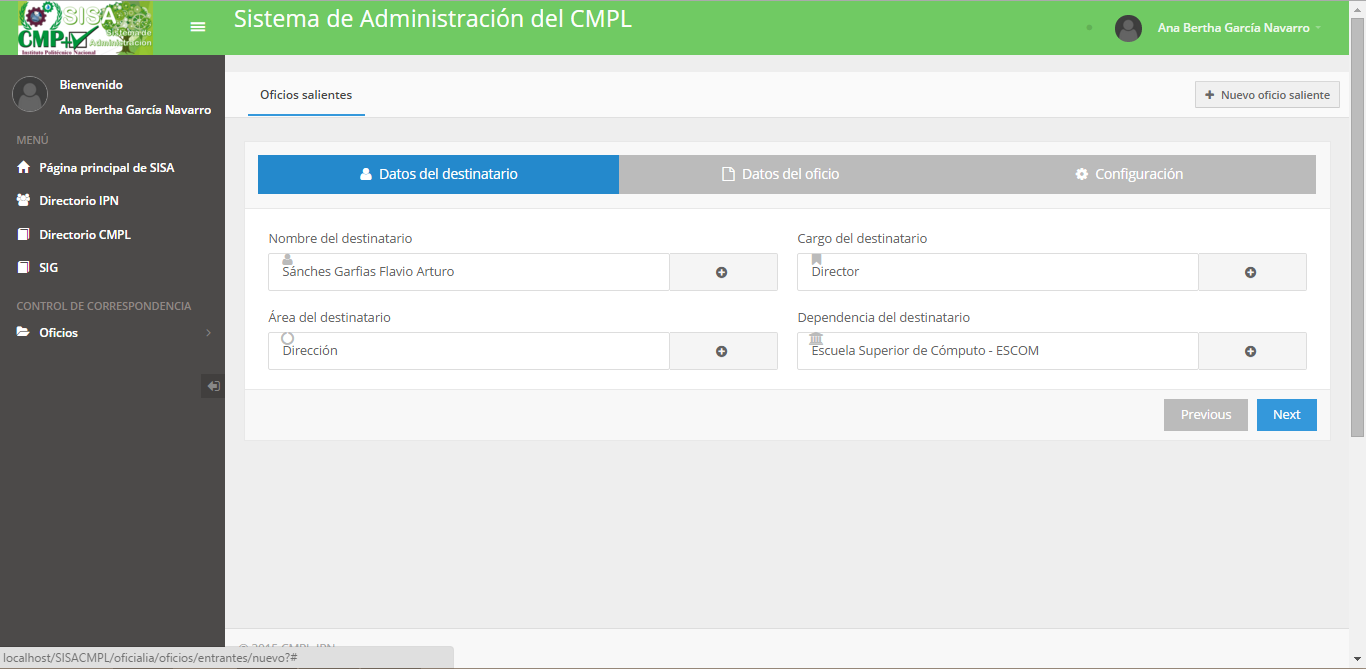
\includegraphics[width=1\textwidth]{Pantallas/Wizard1DatosDelDestinatario.png}
		\caption{Pantalla de datos del remitente de oficios entrantes.}
		\label{fig:Wizard1DatosDelDestinatario}
	\end{figure}

\subsubsection{Funcionamiento}
	Esta pantalla funciona de la siguiente manera:
	
	\begin{enumerate}
		\item La aplicación muestra catálogos para elegir el destinatario, su cargo, su área y su dependencia.
		\item El usuario selecciona de los catálogos la información requerida.
		\item Si el usuario no llegara a encontrar la información deseada, puede darla de alta haciendo clic en ``+'' del tipo de información nueva que desea registrar.
		\item El usuario da clic en ``Next''.
	\end{enumerate}

\subsubsection{Problemas que resuelve}
Esta pantalla ayuda a mitigar las causas que dan origen a los siguientes problemas:

	\begin{itemize}
		\item Es complicado organizar los oficios salientes por dependencias, áreas o departamentos de las entidades que emiten.
		\item No se sabe cuales son las dependencias con las cuales se ha tenido interacción
	\end{itemize}

\subsubsection{Pantallas relacionadas}
Está pantalla se relaciona con las siguientes figuras de pantallas:
	\begin{itemize}
		\item \ref{fig:Wizard2DatosDelOficio}
		\item \ref{fig:NuevoEmisor}
		\item \ref{fig:NuevoCargoEmisor}
		\item \ref{fig:NuevaAreaEmisor}
		\item \ref{fig:NuevaDependencia}
	\end{itemize}
	
%-----------------------------------------------------------------------
\subsection{Pantalla de datos del emisor de oficios entrantes}
\subsubsection{Descripción}
%Descripción amplia de las funciones de la pantalla incluyendo la descripción de todos los botones y las validaciones con las que cuenta
	En esta pantalla el usuario obtendrá de forma automática el identificador de l oficio que le corresponde de manera consecutiva, se especifica quién es el remitente, la fecha de emisión y el asunto. La figura \ref{fig:Wizard2DatosDelOficioSaliente} muestra el diseño de esta pantalla.		
		
	\begin{figure}[htbp!]
		\centering
			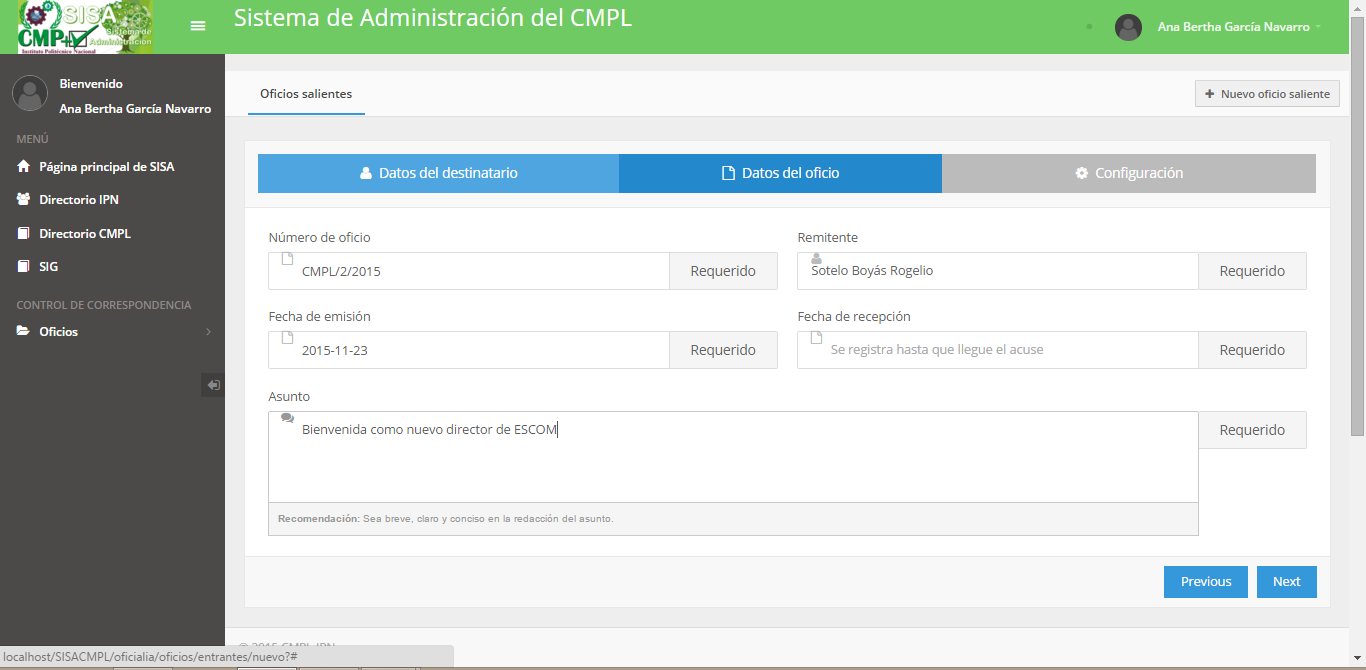
\includegraphics[width=1\textwidth]{Pantallas/Wizard2DatosDelOficioSaliente.png}
		\caption{Pantalla de datos del emisor de oficios entrantes.}
		\label{fig:Wizard2DatosDelOficioSaliente}
	\end{figure}

\subsubsection{Funcionamiento}
	Esta pantalla funciona de la siguiente manera:
	
	\begin{enumerate}
		\item La aplicación genera en automático el identificador del oficio.
		\item El usuario ingresa los datos soliticados por la aplicación en esta pantalla.
		\item El usuario da clic en ``Next''.
	\end{enumerate}

\subsubsection{Problemas que resuelve}
Esta pantalla ayuda a mitigar las causas que dan origen a los siguientes problemas:

	\begin{itemize}
		\item No se sabe cual es el último identificador de oficio usado.
		\item Existen oficios que se redactan con el mismo identificador de oficio.
		\item El registro de oficios no se realiza de forma correcta.
	\end{itemize}

\subsubsection{Pantallas relacionadas}
Está pantalla se relaciona con las siguientes figuras de pantallas:
	\begin{itemize}
		\item \ref{fig:Wizard1DatosDelDestinatario}
		\item \ref{fig:Wizard3ConfiguracionSaliente}
	\end{itemize}

%-----------------------------------------------------------------------
\subsection{Pantalla de configuración de oficios entrantes}
\subsubsection{Descripción}
%Descripción amplia de las funciones de la pantalla incluyendo la descripción de todos los botones y las validaciones con las que cuenta
	En esta pantalla el usuario podrá configurar una fecha en específico de límite de respuesta en caso de que el oficio saliente lo requiera. De igual manera deberá subir el archivo en formato PDF del oficio que redactó para que posteriormente sea revisado y aprobado por oficialía de partes. La figura \ref{fig:Wizard3ConfiguracionSaliente} muestra el diseño de esta pantalla.		
		
	\begin{figure}[htbp!]
		\centering
			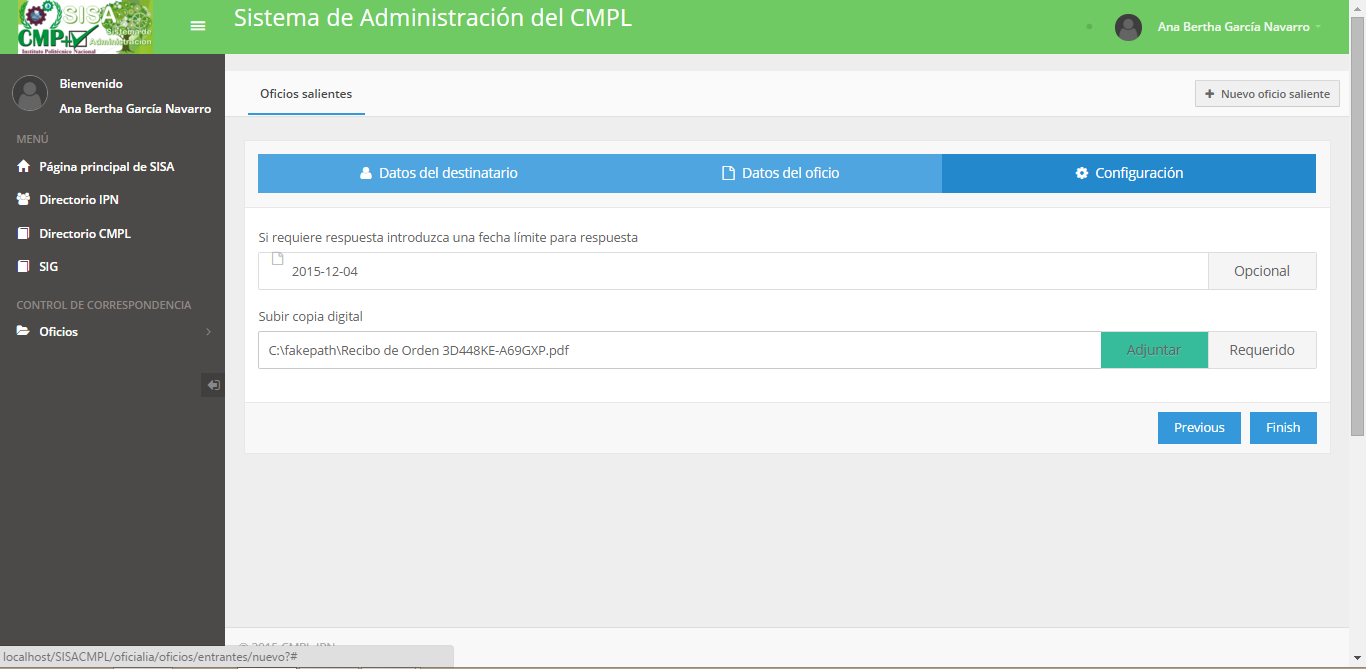
\includegraphics[width=1\textwidth]{Pantallas/Wizard3ConfiguracionSaliente.png}
		\caption{Pantalla de configuración de oficios entrantes.}
		\label{fig:Wizard3ConfiguracionSaliente}
	\end{figure}

\subsubsection{Funcionamiento}
	Esta pantalla funciona de la siguiente manera:
	
	\begin{enumerate}
		\item La aplicación muestra la pantalla para registrar una facha límite de respuesta y adjuntar el archivo con el oficio redactado.
		\item Si el oficio saliente requiere fecha límite de respuesta, el usuario debe seleccionar una fecha de respuesta.
		\item El usuario da clic en "Subir copia digital".
		\item La aplicación muestra una ventana para seleccionar el archivo deseado a subir.
		\item El usuario da clic en "Finish".
	\end{enumerate}

\subsubsection{Problemas que resuelve}
Esta pantalla ayuda a mitigar las causas que dan origen a los siguientes problemas:

	\begin{itemize}
		\item No se tiene un control en la bitácora de registro de los oficios.
		\item No se sabe cuales fueron los oficios registrados debido a que la bitácora no está disponible.
		\item Se gasta papel en la impresión de los oficios que son pasados a revisar por oficialía de partes.
		\item No se sabe cuál es la fecha límite para dar respuesta a un oficio saliente.
		\item No todos los oficios salientes son registrados en la bitácora.
	\end{itemize}

\subsubsection{Pantallas relacionadas}
Está pantalla se relaciona con las siguientes figuras de pantallas:
	\begin{itemize}
		\item \ref{fig:Wizard1DatosDelDestinatario}
		\item \ref{fig:Wizard2DatosDelOficioSaliente}
	\end{itemize}